% Checked drafting: method, simulated results, analyses. Included from main.tex.
% Numbers: results/checked/{main_table.csv, wordtrie.csv, where_saved.json, gain_by_share.csv, extra.json}
% (scripts/run_checked_sim.py, scripts/feasibility/checked_wordtrie.py, scripts/checked_analysis.py).
%=====================================================================
\section{Checked drafting}
\label{sec:checked}

The heads of Section~\ref{sec:method} append their proposals to the draft unchecked, so a wrong head
token reaches the target and ends the round. Yet the draft model reads those proposals anyway in its
next call (cost $c\,r(1+q)$ with $r\approx1$), and that forward also gives the draft's own prediction
after every token it reads. Checked drafting uses this to filter proposals before the target sees them.

\paragraph{Mechanism.} A draft call reads the pending token together with a proposal
$F=(f_1,\dots,f_q)$ and computes its argmax $\hat y_1,\dots,\hat y_{q+1}$ at all $q+1$ positions. It keeps
the longest prefix $f_1,\dots,f_m$ with $f_j=\hat y_j$, appends its own next token $\hat y_{m+1}$, and
crops the rejected proposal tokens from its KV cache. Every drafted token is therefore the draft's own
greedy token: the chain offered to the target is the one plain drafting would produce, but $m$ of its
tokens cost no draft call of their own. The entropy rule is evaluated on the last token of each call and
only decides whether another call is made; tokens a call has already produced are kept. The cost
$r(q)$ was measured with LM-head logits at every position read, so scoring the proposal is included.
The target verifies as before and the output is unchanged. This is the \emph{vertical cascade} of
\citet{chen2024cascade} and \citet{spector2023staged}, with our 1B as the reviewing draft
(Section~\ref{sec:related}).

\paragraph{Proposal sources.}
\begin{itemize}
  \item \textbf{4-gram.} A token 4-gram from 190k IITB Hindi sentences (10.5M Llama-3 tokens): the
  most frequent next token after the longest context (four tokens down to one) seen at least twice,
  applied greedily for up to $L$ tokens. The table takes 6\,MB and a lookup 0.05\,ms on the CPU,
  against 23\,ms for a draft call. It needs no training and knows nothing about words.
  \item \textbf{Heads.} The continuation-vocabulary chain of V0 or V1, read from the hidden state of the
  last token of the previous call and cut at head probability $\tau_h$; the first call of a round has no
  head proposal. The Devanagari gate and the head cost ($0.018\,c$ per call) are as in
  Section~\ref{sec:method}.
  \item \textbf{Both.} The heads' tokens, extended by the 4-gram to $L$ tokens.
\end{itemize}
$\lambda$, $L\in\{4,6,7\}$ and $\tau_h$ are tuned on dev. As further proposers we test a word trie
built from the same corpus, which completes the current word (optionally conditioned on the previous
word, and also proposing the most frequent next word), and, as a bound, the rest of the word the draft
itself will write.

\paragraph{Simulation.} The recorded draft argmax along $y$ tells which proposal tokens the draft
accepts, so rounds and draft calls are exact while the draft is on the target's path. After a wrong
draft token we propose nothing and charge a full call per further token, which is conservative (those
tokens are rejected anyway). Section~\ref{sec:real} tests the simulation against a real decoding loop.

\begin{table}[t]
\centering
\small
\begin{tabular}{lcc}
\toprule
drafter & speed-up [95\% CI] & $\Delta$ vs.\ Entropy [95\% CI] \\
\midrule
Entropy & 1.452 [1.444, 1.461] & --- \\
Heads V1 + lexicon filter, unchecked & 1.542 [1.530, 1.555] & $+0.090$ [$+0.084$, $+0.097$] \\
\midrule
\multicolumn{3}{l}{\emph{checked by the draft model:}} \\
Heads V0 & 1.568 [1.556, 1.581] & $+0.116$ [$+0.112$, $+0.121$] \\
Heads V1 & 1.572 [1.560, 1.586] & $+0.120$ [$+0.115$, $+0.125$] \\
Word trie, current word & 1.582 [1.570, 1.594] & $+0.130$ [$+0.126$, $+0.134$] \\
Word trie + previous word + next word & 1.659 [1.646, 1.673] & $+0.207$ [$+0.202$, $+0.213$] \\
\textbf{4-gram (no training)} & \textbf{1.701 [1.687, 1.716]} & $\mathbf{+0.249}$ [$+0.242$, $+0.256$] \\
4-gram + heads V0 & 1.708 [1.694, 1.724] & $+0.257$ [$+0.249$, $+0.264$] \\
4-gram + heads V1 & 1.705 [1.690, 1.720] & $+0.253$ [$+0.246$, $+0.260$] \\
\midrule
Bound: the draft's own word completion & 1.857 [1.841, 1.875] & $+0.406$ [$+0.395$, $+0.415$] \\
Ceiling: free continuations ($\kappa=0.05$) & 1.911 [1.894, 1.931] & $+0.459$ [$+0.449$, $+0.470$] \\
\bottomrule
\end{tabular}
\caption{Checked drafting, simulated on FLORES devtest (1{,}012 sentences), tuned on dev. The
unchecked heads are the best system of Section~\ref{sec:results}. Heads trained on 180k pairs. The
bound proposes the rest of the word the draft itself will write. $\Delta$: paired bootstrap.}
\label{tab:checked}
\end{table}

\paragraph{Being checked matters more than the proposer.} Table~\ref{tab:checked} gives the results.
Checking alone lifts the V1 heads above the paper's best unchecked system (V1 + lexicon filter) by
$+0.030$ [$+0.024$, $+0.035$]. The training-free 4-gram is far ahead of every head system: $+0.159$
[$+0.151$, $+0.166$] over V1 + lexicon and $+0.129$ [$+0.123$, $+0.135$] over checked V1 heads. On top
of the 4-gram, heads add only $+0.008$ [$+0.006$, $+0.009$] (V0) or $+0.004$ [$+0.002$, $+0.006$] (V1),
and nothing at all on hardware (Section~\ref{sec:real}). Word tries, whose proposals are always real
words, also stay below the 4-gram. Once the draft model checks every proposal, a wrong proposal costs
almost nothing, so what counts is how much a proposer covers, not how often it is right: in the real
loop the 4-gram proposes 8.8 tokens per round and the draft accepts 10\% of them, while the checked V1
heads propose 2.3 tokens per round and the draft accepts 22\%. The heads propose at most $K=3$
continuation tokens inside a word and not at the first call of a round; the 4-gram proposes up to seven
tokens, across word boundaries. Word knowledge (V1's training, the lexicon, a word trie) pays off when
proposals are unchecked, where a wrong token is expensive, and matters little once they are checked.
The bound in Table~\ref{tab:checked} (1.857\x) shows that better proposers could still gain.

\paragraph{The saved calls are word continuations.} Of the draft calls that the 4-gram saves, 77.4\%
are on word-continuation tokens, although only 59.4\% of all tokens, and 64.8\% of the tokens the draft
predicts correctly, are continuations. The gain also grows with how taxed a sentence is
(Figure~\ref{fig:checked_share}): over devtest quintiles of continuation-token share, the gain over
Entropy rises from 14.5\% to 18.8\% (19.1\% in the fourth quintile; Spearman $\rho=0.21$). The same
analysis for V1 + lexicon gives 5.5\% to 8.2\% ($\rho=0.14$). The 4-gram mostly collects the refund of
Section~\ref{sec:feasibility}: once a word has started, its continuation is easy to guess, and the draft
confirms the guess in a call it makes anyway.

\begin{figure}[t]
\centering
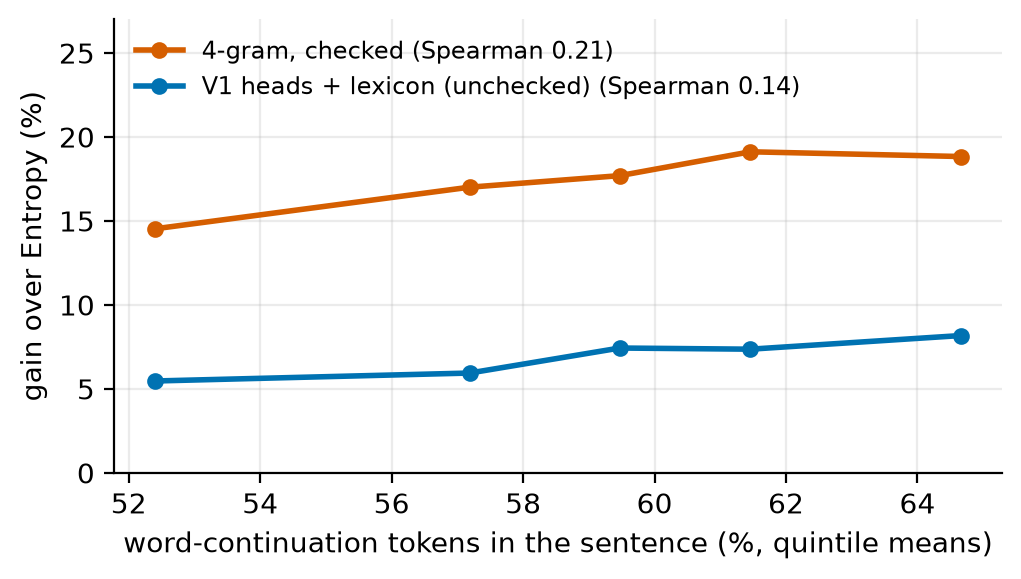
\includegraphics[width=0.7\linewidth]{fig_checked_share.png}
\caption{Gain over Entropy by sentence continuation-token share (devtest quintiles, simulated).}
\label{fig:checked_share}
\end{figure}

\paragraph{Little data, robust to overhead.} The 4-gram needs little data
(Figure~\ref{fig:checked_data_cost}, left): 1k sentences already give 1.615\x, and a 4-gram from only
the 997 dev outputs of the target, without any external corpus, gives 1.660\x. If a call that reads a
proposal cost 5, 10 or 20\% more than measured, the 4-gram would still reach 1.677\x, 1.654\x{} and
1.610\x{} (Figure~\ref{fig:checked_data_cost}, right), above every unchecked head system. The real loop
shows that the measured cost holds.

\begin{figure}[t]
\centering
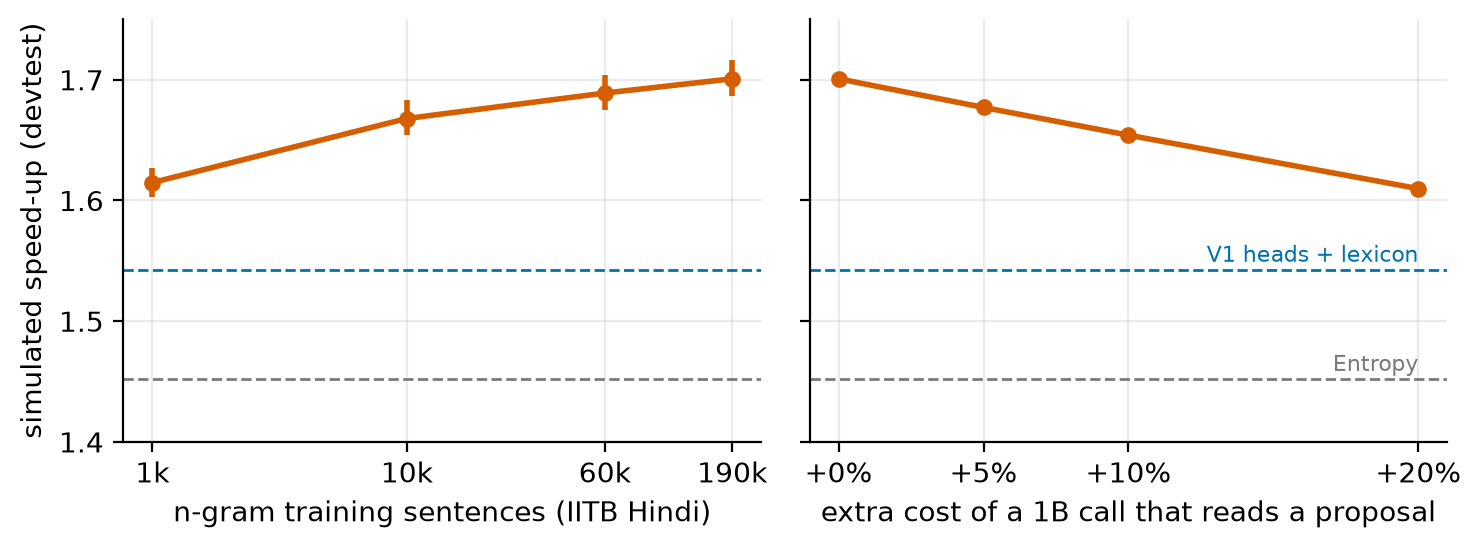
\includegraphics[width=0.9\linewidth]{fig_checked_data_cost.png}
\caption{Checked 4-gram, simulated devtest speed-up. Left: n-gram training sentences (95\% CIs).
Right: extra cost of a draft call that reads a proposal. Dashed: Entropy and V1 heads + lexicon filter.}
\label{fig:checked_data_cost}
\end{figure}
